\label{subsec:output_selection}

\begin{figure}
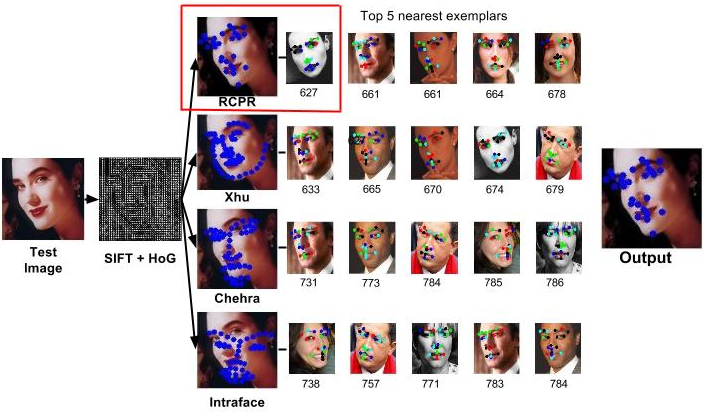
\includegraphics[width=6in, height=3in]{fid/figures/knn_example.png}
\caption{Figure shows how the best solution is selected by using kNN. It shows the top 5 nearest exemplars for each candidate algorithm. Observe if the fiducials are off, the nearest exemplar tend to be dissimilar to the input image.}
\label{fig:knn_example}
\end{figure}

\begin{algorithm}[!h]
\caption{Algorithm for Output Selection by KNN}
\begin{algorithmic}
  \INPUT Training image data $\mathcal{D}$, testing image data $\mathcal{T}$, training
  fiducials $\mathcal{F}_d$, testing fiducials $\mathcal{F}_t$.
  \STATE $\mathcal{E}$ = {\tt ComputeDatasetExemplars}( $\mathcal{D}$, $\mathcal{F}_d$ )
  \STATE $F_{out} = \varnothing$
  \FOR{Each image-fiducial pair $(I,F)$ in $\mathcal{T}$, $\mathcal{F}_t$}
    %\STATE $Face_{size}$ = Bounding box of ground truth annotations in $I$ + $15\%$ more width/height.
    \STATE $I_{face}$ = {\tt CropAndResize}( $I$, $F$ )
    % \STATE $I_{face}$ = {\tt CropFaceResize}( $I$, $Face_{size}$ )
    % \STATE $I_{res}$ = {\tt ImResize}( $I_{face}$, $300 \times 300$ )
    \STATE $\mathcal{O}_{all}$ = {\tt AllFidDetectAlgos}( $I_{face}$ )
    \FOR{ All results $F_i$ in $\mathcal{O}_{all}$ }
      \STATE $Feat_{test}$ = {\tt ComputeFeatures}( $I_{face}$, $F_i$ )
      \FOR{ Each pair $(I_{e}, Feat_{e})$ in $\mathcal{E}$ }
        \STATE $dist_{i, e}$ = {\tt DistFunc}( $Feat_{e}$, $Feat_{test}$ )
      \ENDFOR
      \STATE $dist_i$  = $\arg\min_e dist_{i, e}$
    \ENDFOR
    \STATE $\{ dist_{min}, \quad i \}$ = $\arg\min_i dist_i$
    \STATE $F_{out} = F_{out} \cup F_i$
  \ENDFOR
  \OUTPUT $F_{out}$
\end{algorithmic}
\label{alg:output_selection}
\end{algorithm}

Once the fiducial detection of the state-of-the-art candidate algorithms are obtained for
an input image, we compute appearance 
vectors for an image patch around each fiducial location. Appearance vectors are represented 
in HOG and SIFT space. 
% Note that the SIFT feature is invariant to scale, 
% rotation and illumination which is important for the case of K-Nearest Neighbor approach. 
We concatenate these features them to form the feature vector.

We then compare these candidate algorithm feature vectors 
to the exemplars chosen from the previous approach,
and choose the candidate algorithm-exemplar image output that minimizes the sum of
euclidean distance between common features (equation~\ref{eq:main_fourth_equation}) and is described in Algorithm\ref{alg:output_selection}. Pictorial
representation of this method with the selected exemplars for each of the candidate algorithm
is shown in figure~\ref{fig:knn_example}
Note that this is a simple kNN based approach,
where k=1. Alternatively, we also consider the idea of selecting individual fiducials
from various candidate algorithm outputs, to form our own facial structure that minimizes
an objective function. This is explained in the following section.

